\hyperdef{}{tilda}{}

\subsection{Phylogenetische Rekonstruktion}

\subsubsection{Innere und äußere Sprachgeschichte}

\paragraph{Georg von der Gabelentz (1840-1893) und die Sprachgeschichte}

\begin{quote}
Der Zweig der Sprachforschung, der uns hier beschäftigt, hat es zunächst
mit den trockensten Einzelthatsachen zu thun: Sind die Sprachen A und B
miteinander verwandt, und in welchem Grade? Giebt es dieses Wort oder
jene Form in der und der Sprache oder in der und der Zeit der
Sprachgeschichte? {[}\ldots{}{]} Welche Gesetzmässigkeit herrscht in den
lautlichen Abweichungen? Besteht im einzelnen Falle Urgemeinschaft oder
Entlehnung?
\href{http://bibliography.lingpy.org?key=Gabelentz1891}{(Gabelentz 1891:
145)}
\end{quote}



\begin{quote}
Alles das klingt und ist auch wirklich sehr trocken. Was die menschliche
Re- de im Innersten bewegt, was sonst die Wissenschaft von den Sprachen
der Völker zu einer der lebensvollsten macht, das tritt hier zunächst
zurück: nur einige ihrer Ausläufer ranken in das Seelen- und Sittenleben
der Völker hinüber. Der einzelsprachliche Forscher kann gar nicht
schnell genug die fremde Sprache in's eigene Ich aufnehmen: der
Sprachhistoriker steht draussen vor seinem Gegenstande: hier der Anatom,
da der Cadaver.
\href{http://bibliography.lingpy.org?key=Gabelentz1891}{(Gabelentz 1891:
145)}
\end{quote}





\begin{quote}
Wir werden, um Missverständnisse zu vermeiden, gut thun, zwischen
äusserer und innerer Sprachgeschichte zu unterscheiden. Die äussere
Geschichte einer Sprache ist die Geschichte ihrer räumlichen und
zeitlichen Verbreitung, ihrer Verzweigungen und etwaigen Mischungen
(Genealogie). Die innere Sprachgeschichte erzählt und sucht zu erklären,
wie sich die Sprache in Rücksicht auf Stoff und Form allmählich
verändert hat.
\href{http://bibliography.lingpy.org?key=Gabelentz1891}{(Gabelentz 1891:
146)}
\end{quote}



\subsubsection{Stammbäume und Wellen}

\paragraph{Bäume}

August Schleicher war eine herausragende Persönlichkeit in der
Geschichte der Linguistik. Wir verdanken ihm insbesondere die sogenannte
\emph{Stammbaumtheorie}, die er in zwei frühen Werken erstmals im Jahre
1853 veröffentlichte
(\href{http://bibliography.lingpy.org?key=Schleicher1853}{Schleicher
1853a},
\href{http://bibliography.lingpy.org?key=Schleicher1853a}{Schleicher
1853b}). Schleichers Theorie zur äußeren Sprachgeschichte war
wahrscheinlich direkt beeinflusst von František Čelakovský (1799 --
1852), den er während einer Professur in Prag kennengelernt hatte, und
der noch vor Schleicher einen ersten Stammbaum der slawischen Sprachen
veröf- fentlichte
(\href{http://bibliography.lingpy.org?key=Celakovsky1853}{Čelakovský
1853}).






\begin{quote}
Die ältesten teilungen des indogermanischen bis zum entstehen der
grundsprachen der den sprachstamm bildenden sprachfamilien laßen sich
durch folgendes schema anschaulich machen. Die länge der linien deutet
die zeitdauer an, die entfernung der- selben von einander den
verwantschaftsgrad.
(\href{http://bibliography.lingpy.org?key=Schleicher1861}{Schleicher
1861: 6})
\end{quote}






\href{img/schleicher1861.jpg}{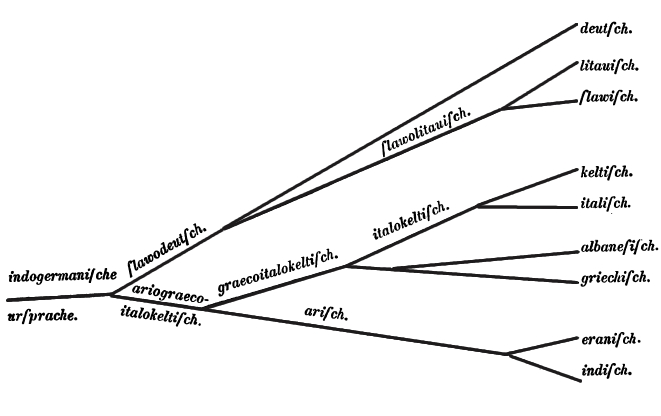
\includegraphics[width=\textwidth]{img/schleicher1861.jpg}}

\href{http://bibliography.lingpy.org?key=Schleicher1861}{Darstellung
aus: Schleicher (1861: 6)}





\paragraph{Wellen}

Nicht lange, nachdem August Schleicher seine berühmte Stammbaumtheorie
erstmals postuliert hatte, regte sich Widerspruch in den Kreisen der
Indogermanisten und histori- schen Linguisten. Am bekanntesten ist in
diesem Zusammenhang das Werk von Johannes Schmidt (1843 -- 1901), der
die Stammbaumtheorie verwarf, und an ihrer Stelle seine nicht minder
berühmte \emph{Wellentheorie} propagierte.






\begin{quote}
Ich möchte an seine stelle das bild der welle setzen, welche sich in
concentrischen mit der entfernung vom mittelpunkte immer schwächer
werdenden ringen ausbreitet. Dass unser sprachgebiet keinen kreis
bildet, sondern höchstens einen kreissector, dass die ursprünglichste
sprache nicht im mittelpunkte, sondern an dem einen ende des gebietes
ligt, tut nichts zur sache. Mir scheint auch das bild einer schiefen vom
sanskrit zum keltischen in ununterbrochener linie geneigten ebene nicht
unpassend.
(\href{http://bibliography.lingpy.org?key=Schmidt1872}{Schmidt 1872:
27})
\end{quote}





\paragraph{Netze und anderes Gewirr}

Das größte Problem von Schmidts Wellentheorie war, das niemand genau
wusste, wie er die äußere Sprachgeschichte denn nun schematisch
darstellen sollte. Und so finden wir im Laufe der Geschichte eine
Vielzahl von Versuchen zur Visualisierung der Wellentheorie.






\href{img/netze.png}{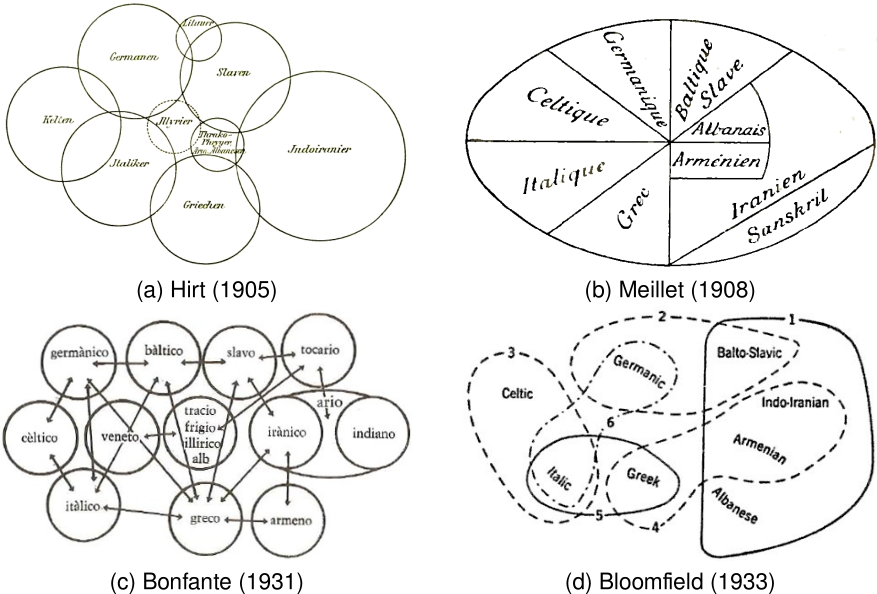
\includegraphics[width=\textwidth]{img/netze.png}}



\subsubsection{\texorpdfstring{{Darstellung und
Analyse}}{Darstellung und Analyse}}

\paragraph{Darstellung von Daten und Darstellung von Geschichte}

Wir müssen unterscheiden zwischen Schemata (seien es Wellen oder Bäume)
zur Darstellung von Daten, und Schemata zur Darstellung von Geschichte
(vgl. die Unterscheidung zwischen data-display und evolutionary in
\href{http://bibliography.lingpy.org?key=Morrison2011}{Morrison 2011:
42f}).





Schleichers Baum von 1861 ist dabei ein klares Beispiel für ein Schema,
das den Anspruch hat, ein geschichtliches Schema zu sein, während die
Beispiele für die Visualisierung der Wellentheorie wohl eher als
Datendarstellungsschemata bezeichnet werden sollten, da sie nicht für
sich in Anspruch nehmen, äußere Sprachgeschichte zu modellieren.
Schemata zur Darstellung von Daten können unter Umständen in Schemata
zur Darstellung von Geschichte überführt werden, jedoch hängt die
Überführbarkeit davon ab, ob die Daten die Rekonstruktion von Geschichte
auch erlauben.




\paragraph{Welche Daten sind es, die auf die Geschichte schließen lassen?}

\begin{quote}
Im ganzen ist also nur wenig, was aus den spezielleren Übereinstimmungen
zwischen einzelnen von den acht Hauptgruppen {[}\ldots{}{]} mit
grösserer Wahrscheinlichkeit entnommen werden kann. Und jedenfalls
treten {[}\ldots{}{]} nirgends speziellere Gemeinsamkeiten, die als
gemeinsame Neuerungen erscheinen, in so grosser Anzahl entgegen, dass
man auf Grund derselben die betreffenden Sprachzweige in derselben Art
zu Einheiten zusammenschliessen dürfte {[}\ldots{}{]}.
(\href{http://bibliography.lingpy.org?key=Brugmann1904}{Brugmann
1904{[}1970{]}: 21f})
\end{quote}

\subsection{Lexikostatistik}

\subsubsection{\texorpdfstring{{Hintergrund und
Grundannahmen}}{Hintergrund und Grundannahmen}}

\paragraph{Hintergrund}

Die Lexikostatistik stellt ein statistisch basiertes Verfahren zur
Ermittlung von Verwandt- schaftsbeziehungen zwischen Sprachen (und damit
zur phylogenetischen Rekonstrukti- on) dar. Sie wurde von Morris Swadesh
(1909 -- 1967) in einer Reihe von Artikeln zu Beginn der 50er Jahre des
20. Jahrhunderts vorgestellt und weiterentwickelt
(\href{http://bibliography.lingpy.org?key=Swadesh1950}{Swadesh 1950},
\href{http://bibliography.lingpy.org?key=Swadesh1952}{Swadesh 1952},
\href{http://bibliography.lingpy.org?key=Swadesh1955}{Swadesh 1955}). In
der Folgezeit mehrte sich jedoch die Kritik an der Methode
(\href{http://bibliography.lingpy.org?key=Bergsland1962}{Bergsland und
Vogt 1962}, \href{http://bibliography.lingpy.org?key=Hoijer1956}{Hoijer
1956}, \href{http://bibliography.lingpy.org?key=Rea1973}{Rea 1973}) und
kam am Ende aus der Mode.




Grundsätzlich werden im Rahmen der Lexikostatistik historisch relevante
Ge- meinsamkeiten zwischen Sprachen ausgezählt. Die zugrunde liegenden
Zahlen können dann weiterverwendet werden, um genealogische Bäume
automatisch zu rekonstruieren, oder um (unter der Annahme konstanten
Wandels) Sprachspaltungszeitpunkte zu ermit- teln. Die Methode erlebte
zu Beginn des 21. Jahrhunderts eine Wiedergeburt im Rahmen neuer
quantitativer biologischer Ansätze, mit deren Hilfe genealogische Bäume
automa- tisch aus spezifischen Sprachdaten gewonnen werden können
(\href{http://bibliography.lingpy.org?key=Atkinson2006}{Atkinson und
Gray 2006}, \href{http://bibliography.lingpy.org?key=Gray2003}{Gray und
Atkinson 2003}).



\paragraph{Grundannahmen}

Die Grundannahmen der Lexikostatistik wurden in einer Vielzahl von
Arbeiten besprochen
(\href{http://bibliography.lingpy.org?key=Gudschinsky1956}{Gudschinsky
1956}, \href{http://bibliography.lingpy.org?key=Sankoff1969}{Sankoff
1969}). Sie lassen sie sich in etwa wie folgt zusammenfassen (vgl.
\href{http://lingulist.de/jump.php?paper=Geisler2014\&href=documents/beautiful_trees.pdf}{Geisler
und List im Erscheinen}):

\begin{itemize}
\item
  The lexicon of every human language contains words which are
  relatively resistant to borrowing and relatively stable over time due
  to the meaning they express: these words constitute the \emph{basic
  vocabulary} of languages.
\item
  \emph{Shared retentions} in the basic vocabulary of different
  languages reflect their degree of \emph{genetic relationship}.
\end{itemize}



\subsubsection{\texorpdfstring{{Praktische
Umsetzung}}{Praktische Umsetzung}}

\paragraph{Die praktischen Arbeitsschritte}

\begin{enumerate}
\itemsep1pt\parskip0pt\parsep0pt
\item
  \textbf{Compilation:} Compile a list of basic vocabulary items (a
  Swadesh-list).
\item
  \textbf{Translation:} Translate the items into the languages that
  shall be investigated.
\item
  \textbf{Cognate Judgments:} Search the language entries for cognates.
\item
  \textbf{Coding:} Convert the cognate information into a numerical
  format.
\item
  \textbf{Computation:} Perform a computational analysis (cluster
  analysis, tree calculation) of the numerical data, which allows to
  make conclusions regarding the phylogeny of the languages under
  investigation.
\end{enumerate}



\paragraph{Diagnostische Testlisten im
\href{http://concepticon.clld.org}{Concepticon}}



\subsubsection{\texorpdfstring{{Kritik}}{Kritik}}

\paragraph{Wichtigste Kritikpunkte in der Literatur}

\begin{itemize}
\itemsep1pt\parskip0pt\parsep0pt
\item
  \textbf{Entlehnung:} Unentdeckte Entlehnungen können die Ergebnisse
  verfälschen.
\item
  \textbf{Aussagekraft:} Lexikalische Ersetzung ist als Prozess nicht
  aussagekräftig für Sprach- geschichte.
\item
  \textbf{Fehleranfälligkeit:} Die Methode ist fehleranfällig, da die
  Daten auf eine problemati- sche Weise erstellt werden.
\end{itemize}




\paragraph{Entscheidender Kritikpunkt}

Neuere Vergleiche haben dabei zeigen können, dass die Daten, die von
Forscherteams unabhängig produ- ziert werden, derartig große
Unterschiede aufweisen, dass dies zu Unterschieden von über 30\% in von
den Daten automatisch berechneten Baumtopologien führt
(\href{http://lingulist.de/jump.php?paper=Geisler2014\&href=documents/beautiful_trees.pdf}{Geisler
und List im Erscheinen}). Die größten Probleme liegen dabei weniger im
Bereich der Kognatenzuweisungen (Schritt 3, obwohl auch dieser
problematisch ist), sondern bereits im Bereich der Überset- zung
(Schritt 2).





Bereits hier zeigen sich große Unterschiede zwischen unabhängig
erstellten Datensätzen, die zeigen, dass mangelnde Kompetenz der
Forscher in den Ein- zelsprachen, aber auch mangelnde Beschreibung der
Konzepte in den Konzeptlisten, zu einer Vielzahl von Unterschieden
bereits in den Ausgangsdaten führen können.



\subsubsection{Komparanda}

\paragraph{Distanzbasierte Ansätze}

Aus den Daten werden Distanzwerte zwischen den zu vergleichenden Taxa
(in unserem Falle Sprachen) abgeleitet. Distanzwerte sind dabei
beliebige Zahlen zwischen $0$ (Identität der Taxa) und
$\textbackslash{}infty$ (Nichtidentität der Taxa), wobei Taxa, die
weiter voneinander entfernt sind, einen größeren Distanzwert zugewiesen
bekommen, als Taxa, die einander näher liegen.

\subsection{Computergestützte Rekonstruktion}


\paragraph{Charakterbasierte Ansätze}

Die Daten werden nicht in Distanzmatrizzen transformiert. Stattdessen
wird jedes Taxon in Bezug auf eine Reihe von Eigenschaften
charakterisiert. Für jede dieser Eigenschaften kann ein Taxon dabei
verschiedene Zustände aufweisen. Die einfachste Zustandsbeschreibung ist
dabei die Anwesenheit oder Ab- wesenheit der jeweiligen Eigenschaft
(dargestellt in einer Binärmatrix). Komplexere Zustände können den Taxa
jedoch ebenfalls zugewiesen werden.




\paragraph{Distanzbasierte versus charakterbasierte Ansätze}

\begin{center}
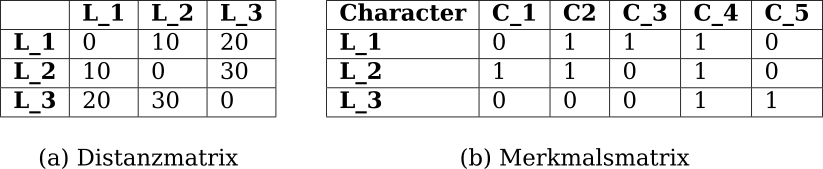
\includegraphics[width=0.5\textwidth]{img/perspective.png}
\end{center}



\subsubsection{\texorpdfstring{{Algorithmen}}{Algorithmen}}

\paragraph{Allgemeines Vorweg}

Um aus den in Distanzform oder Charakterform kodierten Daten mit Hilfe
des Computers einen Stammbaum abzuleiten, müssen diese geclustert
werden. Hierzu sind in der Biologie verschiedene Verfahren entwickelt
worden. Es gibt eine Vielzahl verschiedenster Softwareprogramme, welche
diese Aufgabe erfüllen. Den einzelnen Anwendungen innerhalb dieser
Software liegen dabei verschiedene Algorithmen zugrunde, welche aus den
Daten sukzessive einen Baum erzeugen, oder aus einer Vielzahl möglicher
Bäume den wahrscheinlichsten Baum ermitteln.




\begin{itemize}
\itemsep1pt\parskip0pt\parsep0pt
\item
  \textbf{Neighbor-Joining:} Clusterverfahren für Distanzdaten,
  entwickelt von
  \href{http://bibliography.lingpy.org?key=Saitou1987}{Saitou and Nei
  (1987)}, welches sich insbesondere deshalb großer Beliebtheit erfreut,
  weil es eine sehr geringe Laufzeit hat. Um einen schnellen Überblick
  über die Daten zu bekommen, ist es daher sehr gut geeignet.
\item
  \textbf{Likelihood-Verfahren:} Verfahren für Charakterdaten, die auf
  stochastischen Verfahren beruht und entweder alle möglichen Bäume auf
  ihre Wahrscheinlichkeit vergleichen (``maximum likelihood'',
  \href{http://bibliography.lingpy.org?key=Nunn2011}{Nunn 2011:33-35}),
  oder ein möglichst großes Sample ``guter'' Bäume automatisch schätzt
  (``bayesian methods'',
  \href{http://bibliography.lingpy.org?key=Nunn2011}{Nunn 2011:35-38}).
\item
  \textbf{Maximale Parsimonie:} Verfahren, welches den evolutionären
  Baum errechnet, der am wenigsten evolutionären Wandel benötigt, um die
  Daten zu erklären
  (\href{http://bibliography.lingpy.org?key=Nunn2011}{Nunn 2011:30-33}).
\end{itemize}




\paragraph{Software}

\begin{itemize}
\itemsep1pt\parskip0pt\parsep0pt
\item
  \href{http://lingpy.org}{LingPy}: Bietet distanzbasierte
  Clusterverfahren, unter anderem Neighbor-Joining
  (\href{http://bibliography.lingpy.org?key=Saitou1987}{Saitou und Nei
  1987}) und UPGMA
  (\href{http://bibliography.lingpy.org?key=Sokal1958}{Sokal und
  Michener 1958}).
\item
  \href{http://mrbayes.sourceforge.net}{MrBayes}: Bietet bayesianische
  Methoden, die vor allem in der Biologie verwendet werden
  (\href{http://bibliography.lingpy.org?key=Ronquist2009}{Ronquist et
  al. 2009}).
\item
  \href{http://splitstree.org}{SplitsTree}: Bietet distanzbasierte
  Clusterverfahren, aber vor allem auch distanzbasierte
  Netzwerkanalysen, wie zum Beispiel NeighborNet
  (\href{http://bibliography.lingpy.org?key=Bryant2002}{Bryant und
  Moulton 2002}).
\end{itemize}



\subsubsection{Formate}

\paragraph{Allgemeines Vorweg}

Als Eingabedaten werden in den phylogenetischen Analysen im Rahmen der
histo- rischen Linguistik zumeist Swadesh-Listen (vgl.
\href{http://bibliography.lingpy.org?key=Swadesh1950}{Swadesh 1950},
\href{http://bibliography.lingpy.org?key=Swadesh1952}{1952},
\href{http://bibliography.lingpy.org?key=Swadesh1955}{1955}) verwendet.
Jedes Item (``Bedeutungsslot'') wird dabei zunächst als Charakter
angesehen. Diesem wird für jede Sprache ein Zustand zugewiesen, wobei
der Zustand als identisch kodiert wird, wenn die jeweiligen
Spracheinträge kognat sind.





\paragraph{Distanzberechnung aus Swadeshlisten}

\begin{center}
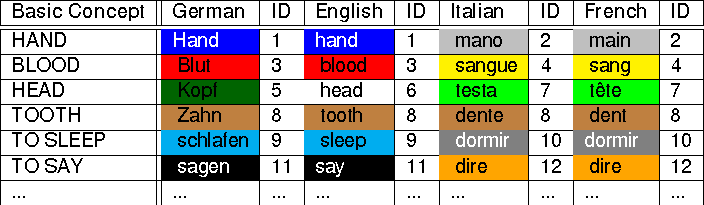
\includegraphics[width=0.5\textwidth]{img/cognates-1.pdf}
\end{center}




\paragraph{Distanzberechnung aus Swadeshlisten}

\begin{center}
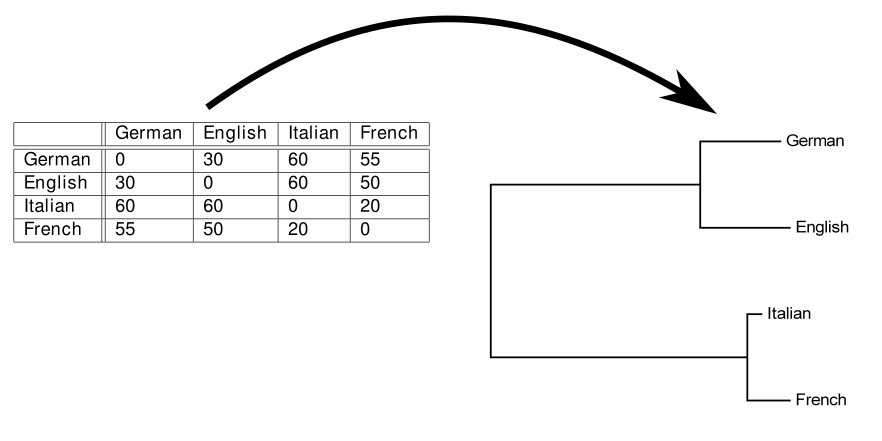
\includegraphics[width=\textwidth]{img/distance-tree.png}
\end{center}




\paragraph{Charaktermodellierung von Kognatensätzen}
\begin{center}
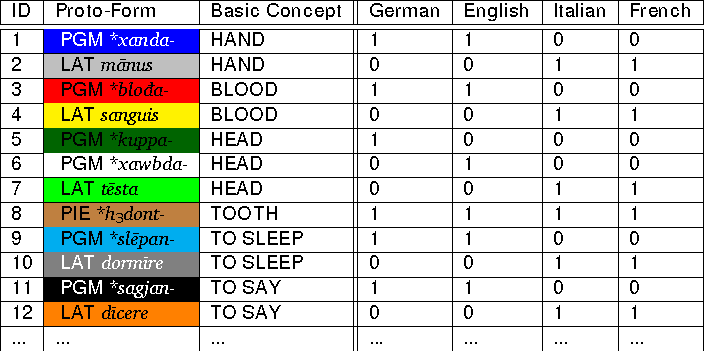
\includegraphics[width=0.5\textwidth]{img/cognates-2.pdf}
\end{center}




\begin{center}
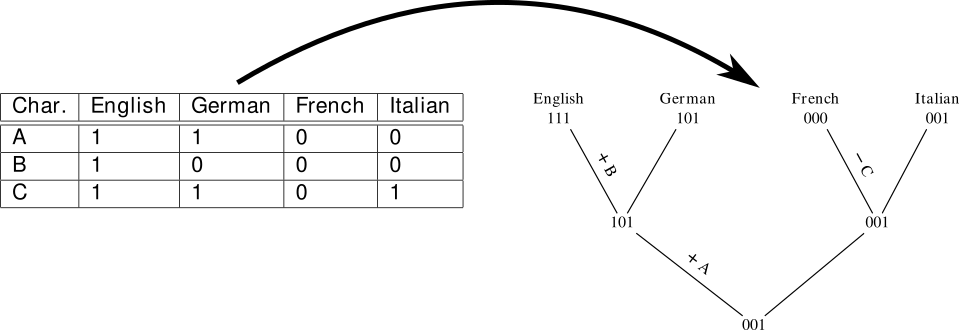
\includegraphics[width=\textwidth]{img/character-tree.png}
\end{center}




\paragraph{Phylip-Format}

\begin{verbatim}
12
Germa 0.0 0.19 0.11 0.27 0.19 0.26 0.16 0.16 0.19 0.22 0.11 0.08
Engli 0.19 0.0 0.14 0.27 0.19 0.22 0.16 0.16 0.26 0.22 0.11 0.14
Dutch 0.11 0.14 0.0 0.29 0.21 0.27 0.14 0.18 0.24 0.24 0.13 0.09
Icela 0.27 0.27 0.29 0.0 0.08 0.21 0.14 0.11 0.27 0.08 0.22 0.22
Nynor 0.19 0.19 0.21 0.08 0.0 0.13 0.06 0.03 0.22 0.06 0.14 0.14
Riksm 0.26 0.22 0.27 0.21 0.13 0.0 0.13 0.09 0.29 0.16 0.21 0.21
Swedi 0.16 0.16 0.14 0.14 0.06 0.13 0.0 0.03 0.19 0.09 0.11 0.11
Danis 0.16 0.16 0.18 0.11 0.03 0.09 0.03 0.0 0.19 0.06 0.11 0.11
Gothi 0.19 0.26 0.24 0.27 0.22 0.29 0.19 0.19 0.0 0.22 0.18 0.18
OIcel 0.22 0.22 0.24 0.08 0.06 0.16 0.09 0.06 0.22 0.0 0.14 0.18
OEngl 0.11 0.11 0.13 0.22 0.14 0.21 0.11 0.11 0.18 0.14 0.0 0.06
OHGer 0.08 0.14 0.09 0.22 0.14 0.21 0.11 0.11 0.18 0.18 0.06 0.0
\end{verbatim}





\paragraph{Nexus-Format}

\begin{verbatim}
#nexus
BEGIN Taxa;
DIMENSIONS ntax=12;
TAXLABELS 'Germa' 'Engli' 'Dutch' 'Icela' 'Nynor' 'Riksm' 'Swedi' 'Danis'
'Gothi' 'OIcel' 'OEngl' 'OHGer';
END; [Taxa]
BEGIN Characters;
DIMENSIONS nchar=61;
FORMAT
datatype=STANDARD
missing=?
gap=-
symbols="01"
labels=left
transpose=no
interleave=no
;
MATRIX
'Germa' 0111111111111111111111111111111111111111100000000000000000000
'Engli' 0100011111111111111011111111010110111111111111000000000000000
'Dutch' 0101111111111111111111111111010111111111110010110000000000000
'Icela' 0100111110111111110111110111011110111111110001001111111100000
AH
'Nynor' 0100111110111111110111111111011110111111110001001110010000000
'Riksm' 0100010110111010111111011111011110111111110001001010010010000
'Swedi' 0100111110111111111111111111011110111111110001101010000000000
'Danis' 0100111110111111111111111111011110111111110001001010010000000
'Gothi' 0100111011111111111101110111011111111111100001001000000001111
'OIcel' 0100111110111111111111111111011110111111110001001111010101000
'OEngl' 0101111111111111111111111111011110111111110101000000000001000
'OHGer' 0101111111111111111111111111011111111111110100001000000000000
;
END;
\end{verbatim}

